\documentclass[12pt,a4paper]{article}

\usepackage{graphicx} % For including images
\usepackage{amsmath} % For mathematical equations
\usepackage{amssymb} % For mathematical symbols
\usepackage{float} % To manage figure positioning
\usepackage{geometry} % For page layout
\usepackage[hidelinks]{hyperref} % For hyperlinks
\usepackage{caption} % For customizing figure captions
\usepackage{multicol} % For multiple columns


% Page geometry
\geometry{margin=0.7in}

% Title
\title{\textbf{Vibrational Analysis with a Focus on Phase-Plane Diagrams}}
\date{\today}

\begin{document}

% Title Page
\maketitle

% Group Members Section
\begin{center}
    \small
    \begin{tabular}{c c c}
        NZAN Davies Ntun (Leader) & NDUKWE Chidubem Emmanuel & OTOIJAGHA Blessing \\
        211605045 & 211605027 & 211605038 \\
        & & \\
        NWAEKE Chimdindu Stephanie & MUKU Wengyam Maryam & JOB-BARNABAS OBUETOR \\
        211605047 & 211605053 & 211605029 \\
        & & \\
        ADESOKAN Bolurin & OLOTU Samuel Kayode & Adepoju Mobolaji Adrain \\
        211605017 & 211605076 & 20221878 \\
        & & \\
        SAMPSON David & USMANN Abdullahi Garba & IFEANYICHUKWU Ejezie \\
        211605020 & 211605024 & 211605039 \\
        & & \\
        MUHAMMAD Yahaya Yahaya & SULAIMAN UmmSalama & Boniface Solomon \\
        211605062 & 211605008 & 211605054 \\
    \end{tabular}
\end{center}

\tableofcontents
\newpage

\section{Part 1: Harmonic Force on the Rocket}
\subsection{System Sketch and Representation}
\begin{figure}[H]
    \centering
    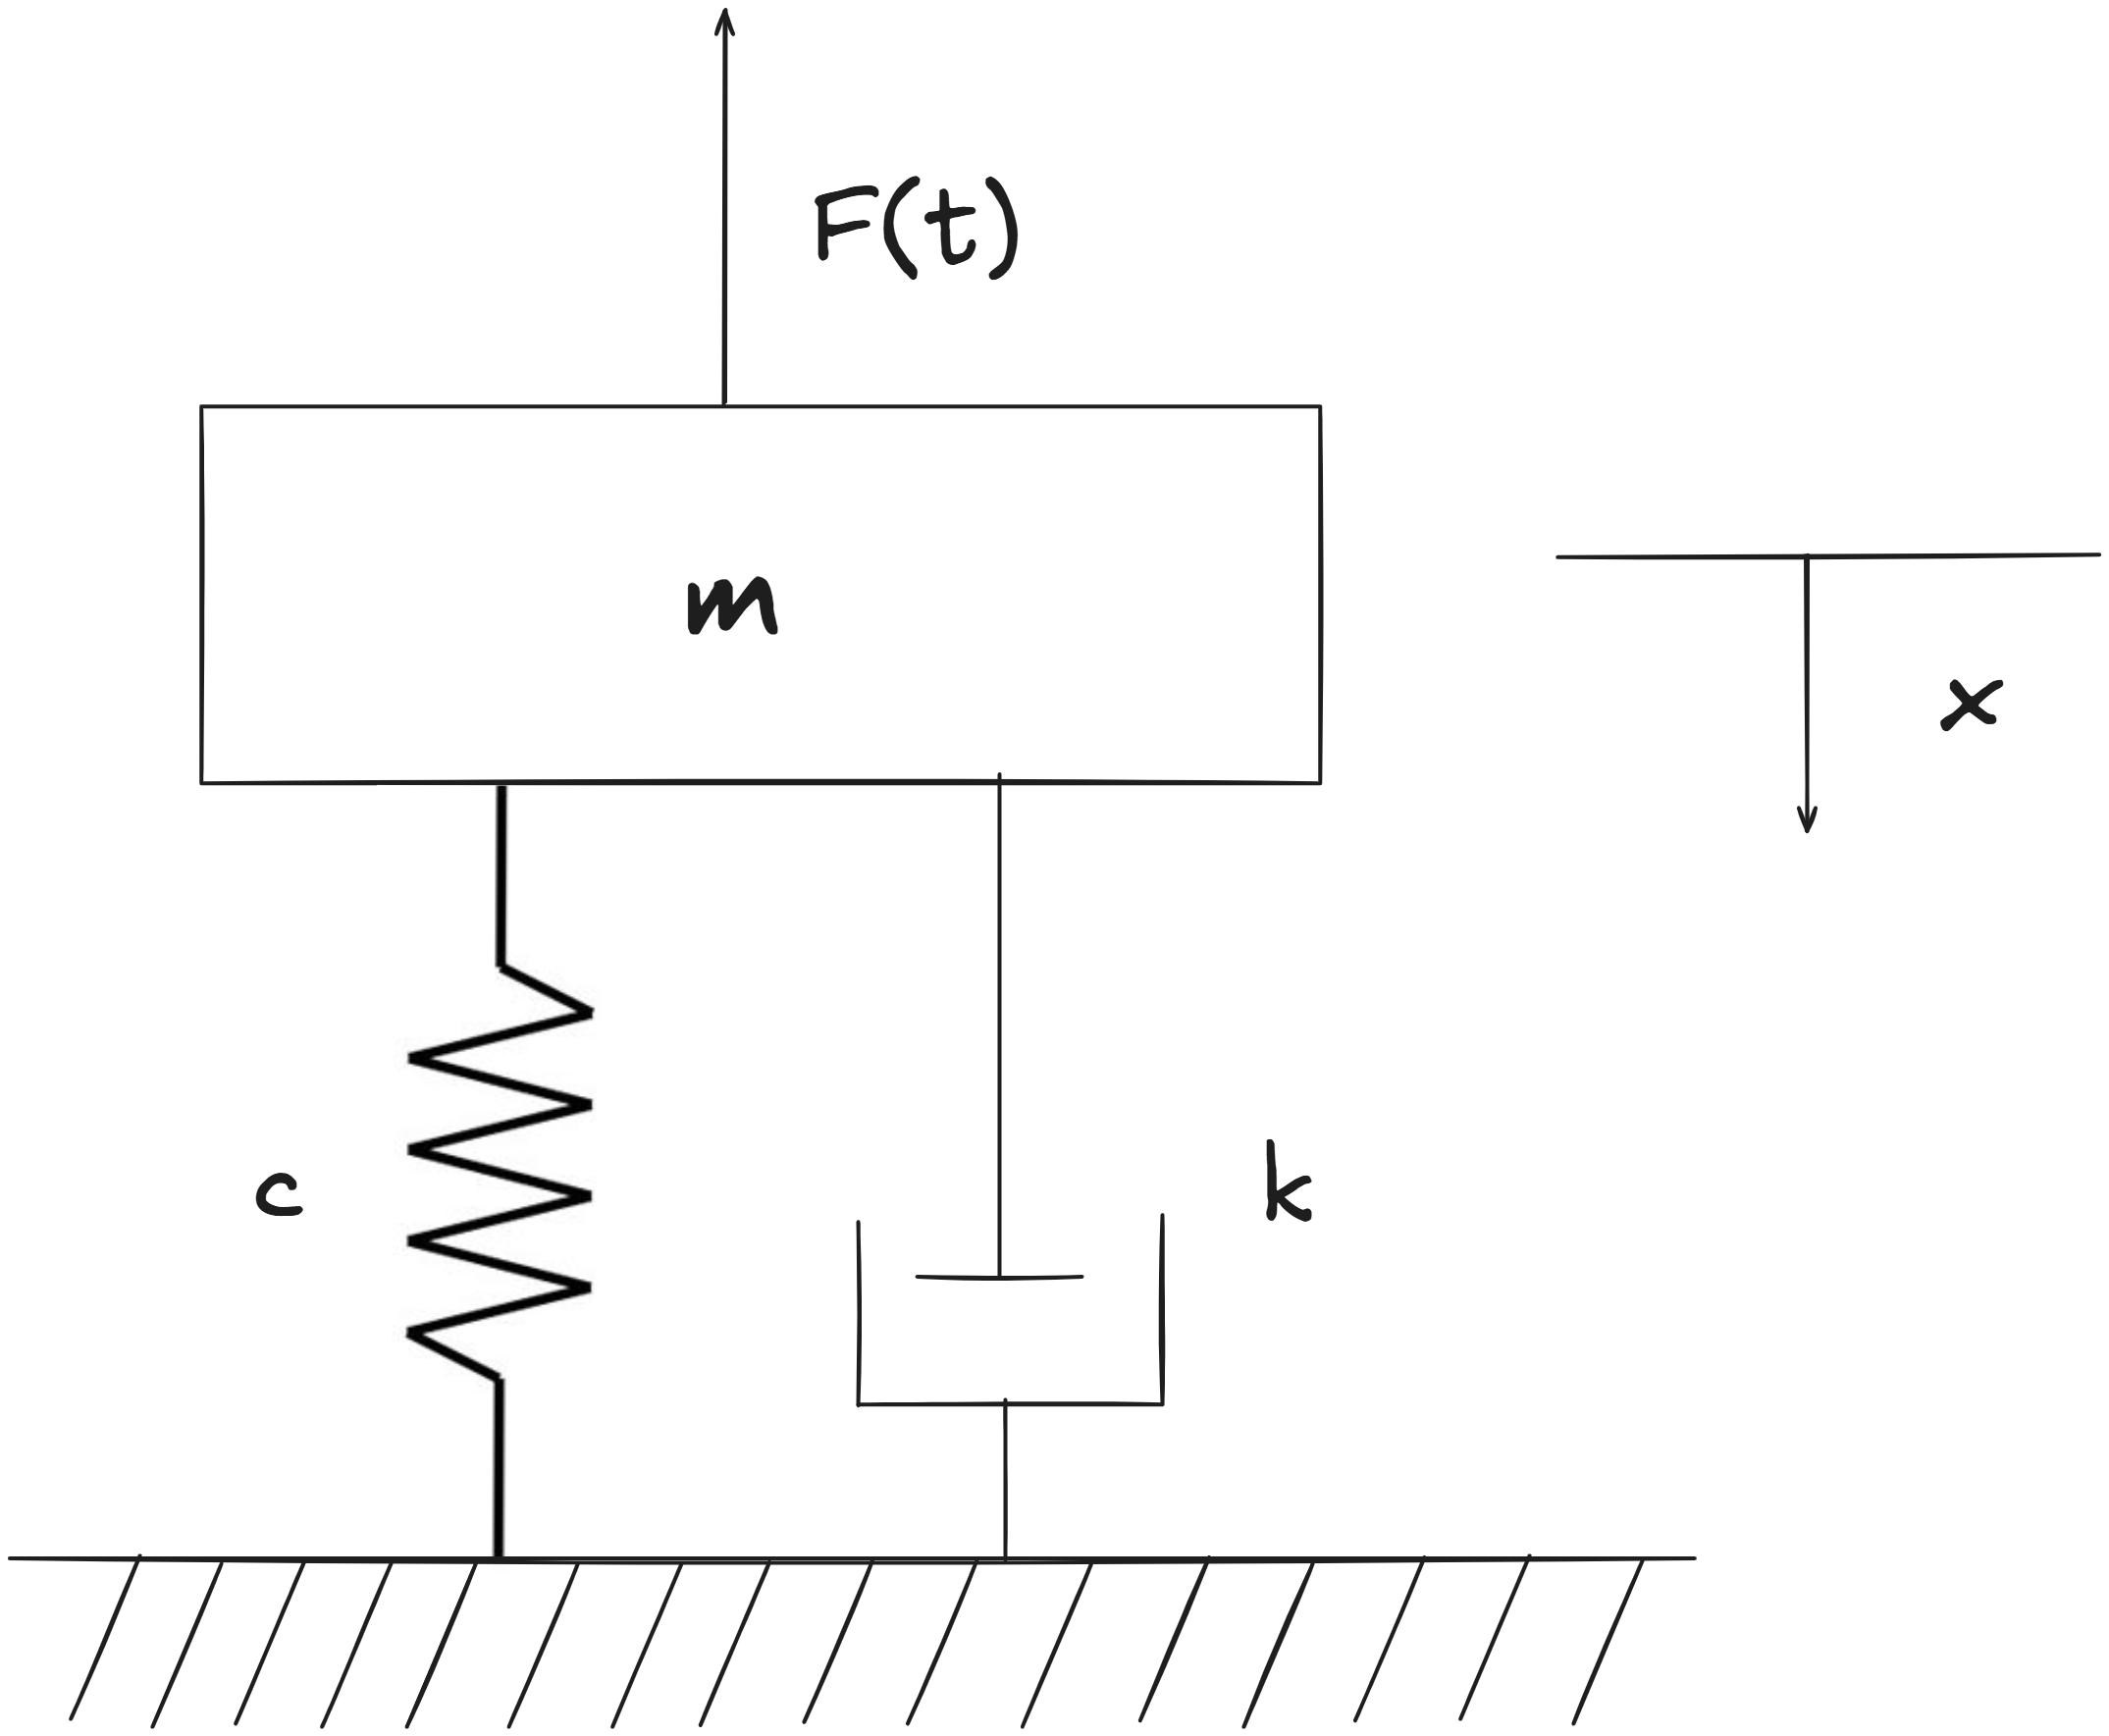
\includegraphics[width=0.8\textwidth]{msd_harmonic.png} 
    \caption{Mass-Spring-Damper System.}
    \label{fig:system}
\end{figure}
\textbf{Where:}
\begin{itemize}
    \item Spring constant, \(c = 20 \, \text{N/m}\)
    \item Damping constant, \(k = 5 \, \text{Ns/m}\)
    \item Mass, \(m = 5 \, \text{kg}\)
    \item Initial position, \(x = 10 \, \text{m}\)
    \item Harmonic Force, \(F(t) = F_0 \cos(\omega t)\)
    \item Angular frequencies, \(\omega = [3, 162, 4.5] \, \text{rad/s}\)
\end{itemize}

\subsection{Hand-Drawn Gaussian Plane: Force Estimation}

\begin{figure}[H]
    \centering
    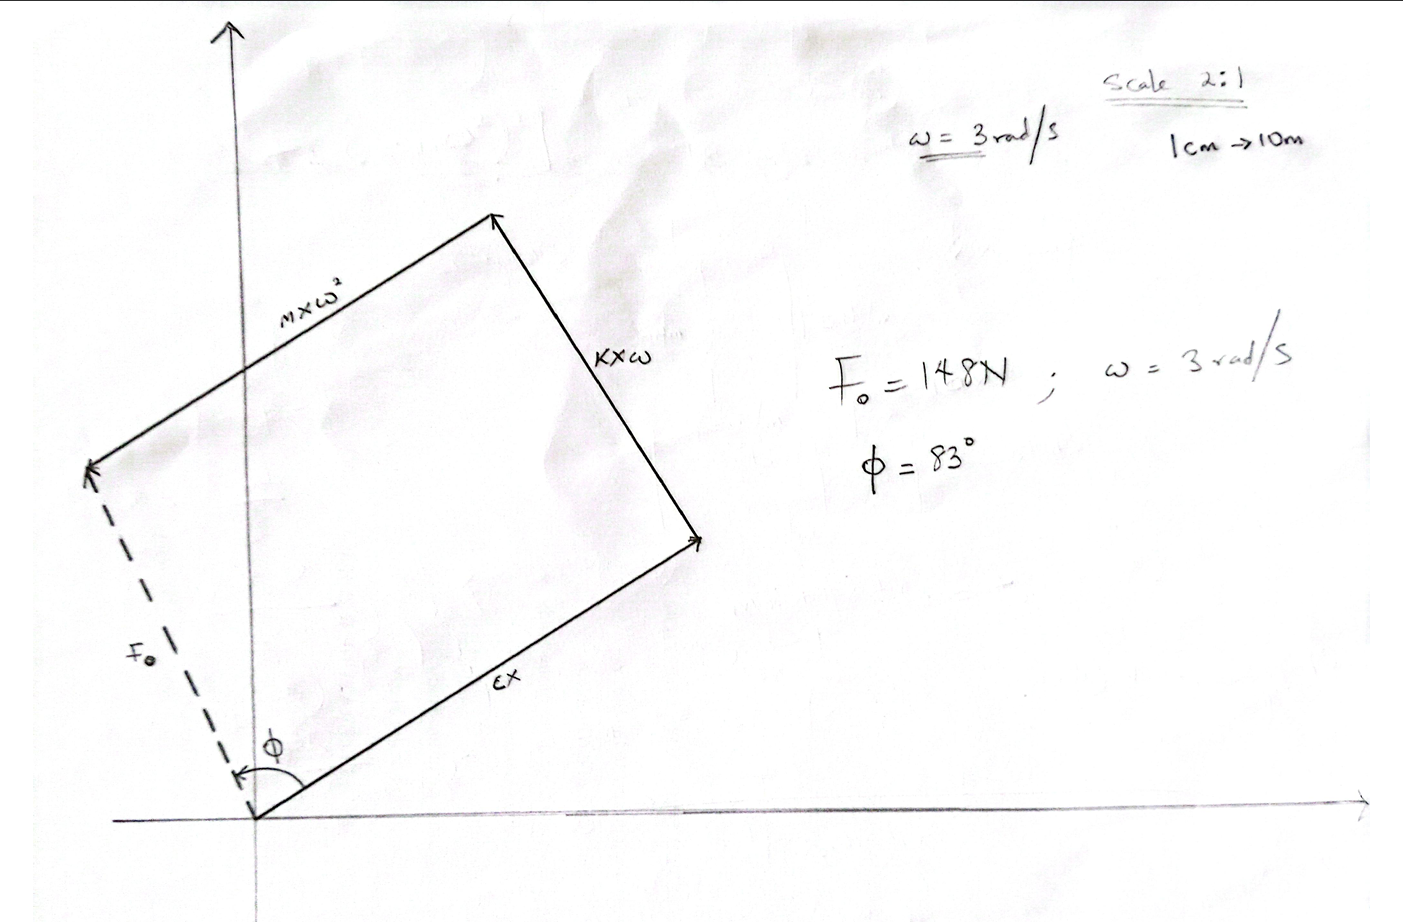
\includegraphics[width=0.8\textwidth]{3rads.png} 
    \caption{Force estimation for $\omega$ = 3 rads/s.}
    \label{fig:system}
\end{figure}

\begin{figure}[H]
    \centering
    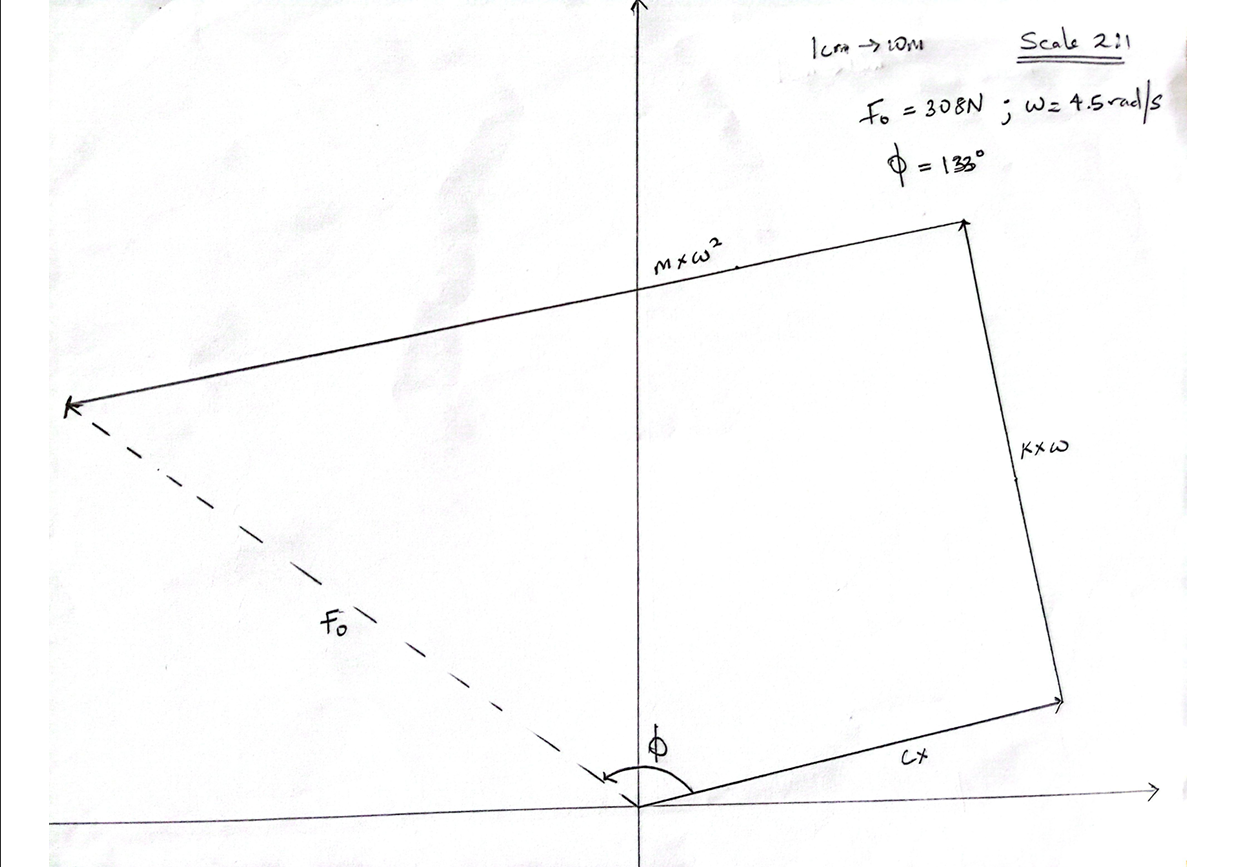
\includegraphics[width=0.8\textwidth]{4.5rads.png} 
    \caption{Force estimation for $\omega$ = 4.5 rads/s.}
    \label{fig:system}
\end{figure}

\begin{figure}[H]
    \centering
    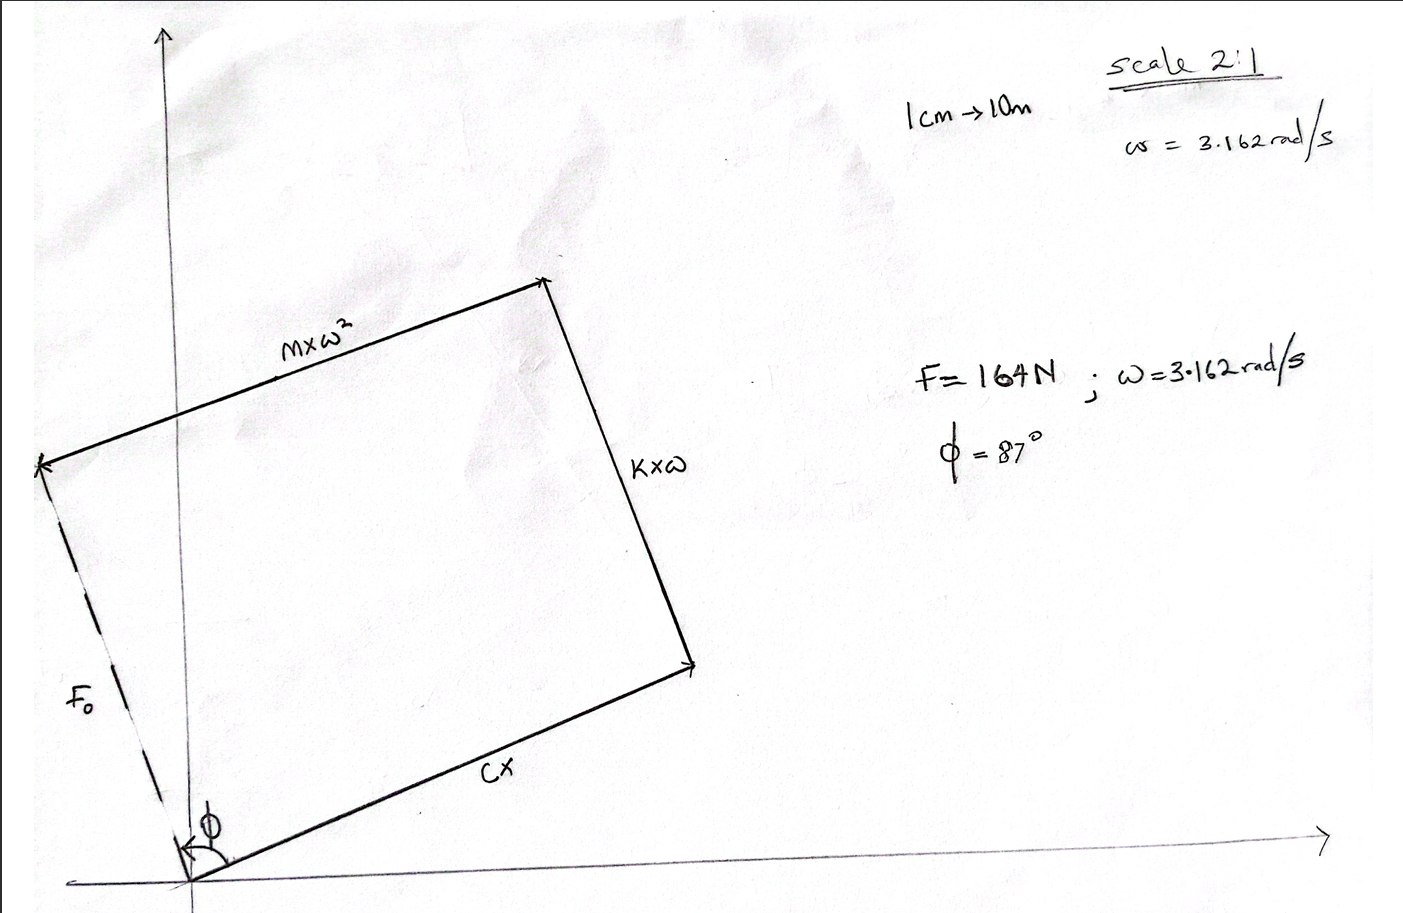
\includegraphics[width=0.8\textwidth]{3.162rads.png} 
    \caption{Force estimation for $\omega$ = 3.162 rads/s.}
    \label{fig:system}
\end{figure}

\begin{figure}[H]
    \centering
    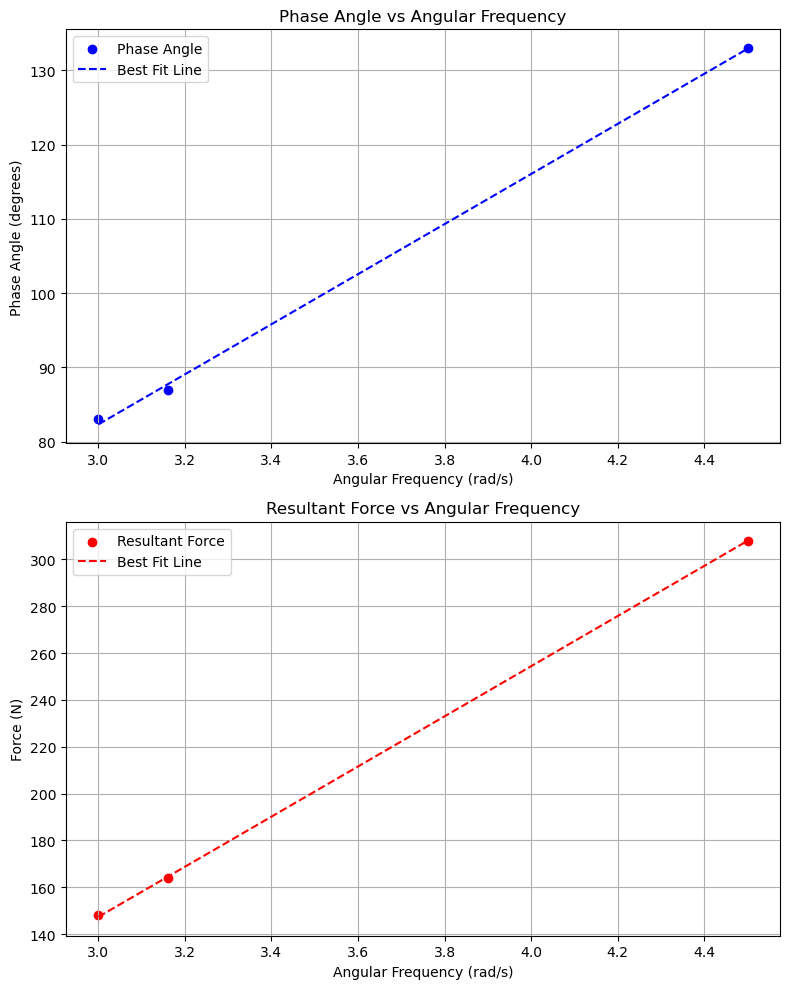
\includegraphics[width=0.8\textwidth]{phase_force_angfreq.png} 
    \caption{Phase angle and Reultanat Force for different Angular Frequencies.}
    \label{fig:system}
\end{figure}

As seen from Fig 5, the phase angle and resultant force are directly proportional to the angular frequency. The phase angle increases as the angular frequency increases, also, the resultant force increases with the angular frequency. This relationship is due to the system's response to the harmonic force, which is influenced by the system's natural frequency and damping ratio.

\subsection{Mathematical Comparison of Forces}

Parameters:
\begin{itemize}
    \item Spring constant, \(c = 20 \, \text{N/m}\)
    \item Damping constant, \(k = 5 \, \text{Ns/m}\)
    \item Mass, \(m = 2 \, \text{kg}\)
    \item Initial position, \(x = 10 \, \text{m}\)
    \item Angular frequencies, \(\omega = [3, 162, 4.5] \, \text{rad/s}\)
\end{itemize}

\noindent\textbf{Amplitude:} 
\[
\hat{X} = \frac{F_{\text{exc}}}{\sqrt{(k \cdot \omega)^2 + (c - m \cdot \omega^2)^2}}
\]

\noindent\textbf{Phase Angle:}
\[
\phi = \tan^{-1} \left( \frac{k \cdot \omega}{c - m \cdot (\omega^2)} \right)
\]

\noindent\textbf{After substituting:}
\begin{itemize}
    \item \(\omega\) = 3 rad/s ; F = 151.33N ; \(\phi\) = 82.4\(^{\circ}\)
    \item \(\omega\) = 3.162 rad/s ; F = 158.1N ; \(\phi\) = 89.9 \(^{\circ}\)
    \item \(\omega\) = 4.5 rad/s ; F = 304.38N ; \(\phi\) = 133 \(^{\circ}\)
\end{itemize}
{\vspace{5pt}}
The mathematical calculations closely match the graphical estimations, confirming the relationship between the system's response and the harmonic force's angular frequency. 

Precision and accuracy are essential in engineering analysis, as small errors can lead to significant deviations in system behavior. By comparing the graphical and mathematical results, engineers can validate their assumptions and ensure the reliability of their designs, here calculations.
{\vspace{5pt}}
\subsection{Discussion of the Gaussian Plane Approach}

The Gaussian plane method provides a visual representation of the system's response to harmonic forces, making it easier to understand the relationship between force amplitude, phase angle, and angular frequency. The graphical estimation closely matches the mathematical computation to some degree, confirming the accuracy of the method in predicting system behavior.

{\vspace{5pt}}

Gaussian plane diagrams are a valuable tool for engineers to quickly estimate system responses and identify trends without complex calculations. By visually analyzing the phase angle and resultant force, engineers can gain insights into how the system behaves under different conditions and make informed design decisions. The method provides a clear and intuitive way to interpret complex data and communicate findings effectively.



{\vspace{5pt}}

\subsection{Damping Ratio and Curl}
\begin{figure}[H]
    \centering
    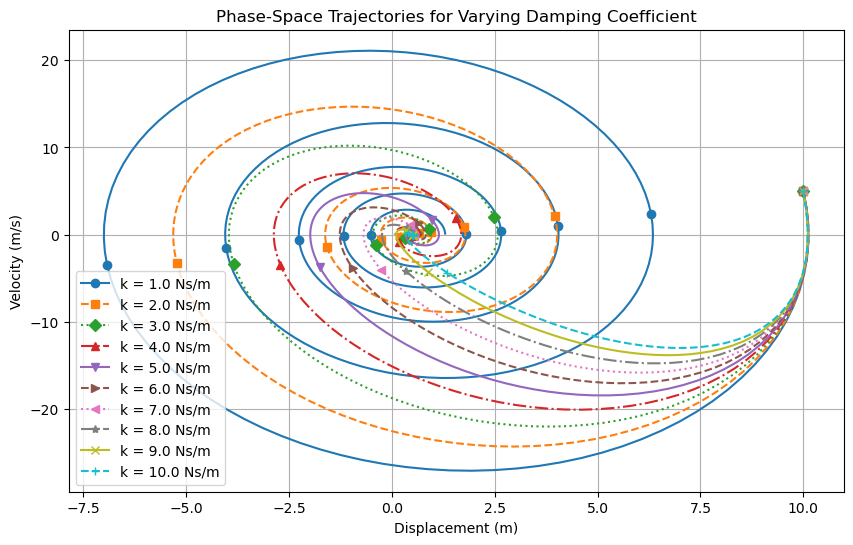
\includegraphics[width=0.8\textwidth]{damping_ratio_to_curl.png} 
    \caption{Phase Trajectory for Varying Damping Coefficient}
    \label{fig:system}
\end{figure}
{\vspace{10pt}}


The phase trajectory for varying damping coefficients shows how the system's response changes based on the damping ratio. The damping ratio affects the system's ability to dissipate energy, influencing the amplitude and phase of the system's response.

For low damping ratios, the system exhibits a curling behavior, where the phase trajectory spirals inward towards the origin. This indicates that the system oscillates with decreasing amplitude over time, eventually reaching a stable equilibrium. The curling behavior is characteristic of underdamped systems, where energy is gradually dissipated due to damping.

As the damping ratio increases, the phase trajectory becomes less curled and approaches a straight line. This indicates that the system's response is more critically damped, reaching equilibrium faster without oscillating. The system's behavior is influenced by the balance between the spring's restorative force, the damping force, and the mass's inertia.

By analyzing the phase trajectory for different damping ratios, engineers can optimize the system's performance by adjusting the damping coefficient to achieve the desired response characteristics. Understanding how damping affects the system's behavior is crucial for designing stable and efficient mechanical systems.

{\vspace{10pt}}

\subsection{Angular Frequency and Its Effect on the System}
\begin{figure}[H]
    \centering
    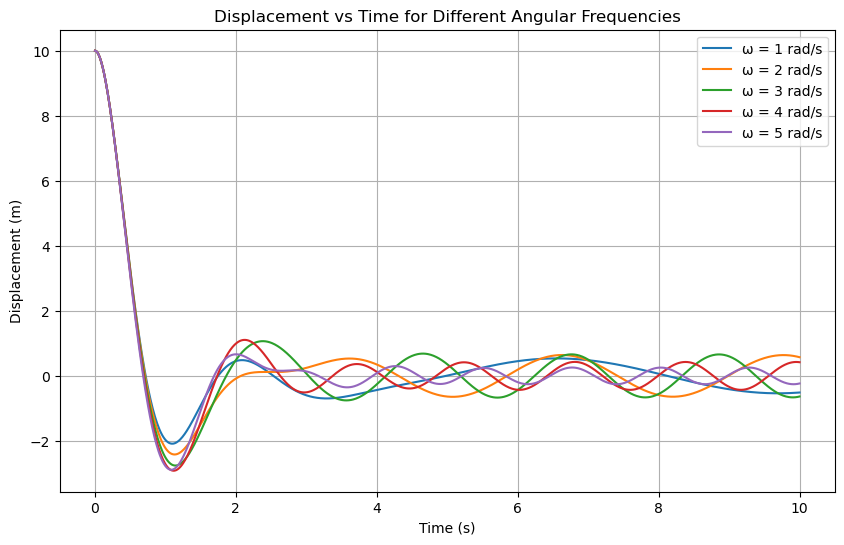
\includegraphics[width=0.8\textwidth]{angular_freq_effect_on_system.png} 
    \caption{Displacement vs Time for Different Angular Frequencies}
    \label{fig:system}
\end{figure}
{\vspace{10pt}}


The graph shows the displacement of the system over time for different angular frequencies. The system's response varies based on the excitation frequency, with higher frequencies leading to faster oscillations and shorter periods. The amplitude of the displacement also changes with the angular frequency, with higher frequencies resulting in larger displacements.

The system's behavior is influenced by the balance between the spring's stiffness, the damping force, and the mass's inertia. At lower frequencies, the system has more time to respond to the excitation, resulting in larger displacements. As the frequency increases, the system's response becomes more rapid, leading to shorter oscillations and smaller displacements.



{\vspace{10pt}}

\subsection{Varying the Spring Constant}
\begin{figure}[H]
    \centering
    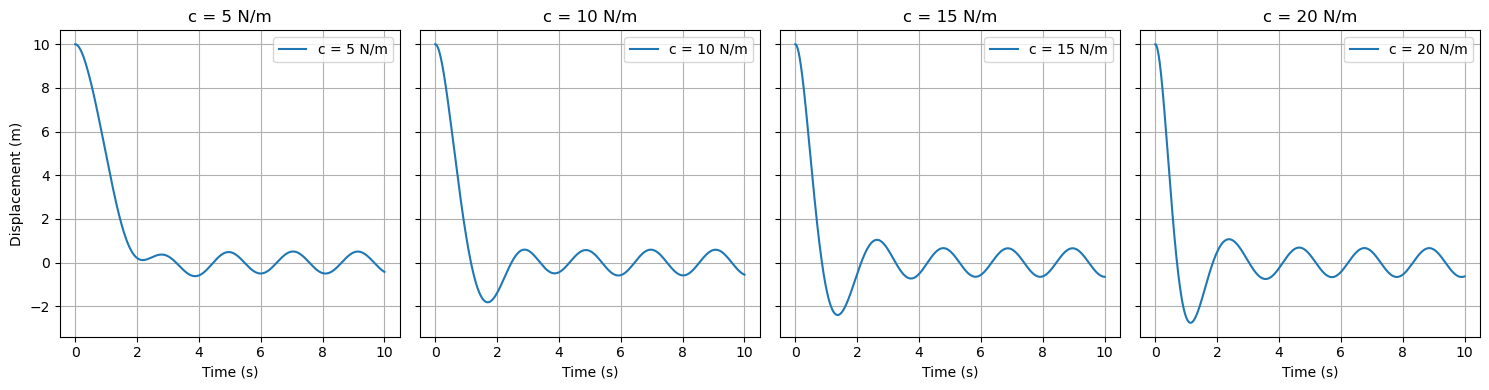
\includegraphics[width=0.8\textwidth]{spring_constant_effect_on_system.png} 
    \caption{Displacement vs Time for Different Angular Frequencies}
    \label{fig:system}
\end{figure}
{\vspace{10pt}}


The graph shows the displacement of the system over time for different spring constants. The spring constant affects the system's stiffness, influencing how the system responds to external forces. A higher spring constant results in a stiffer system, leading to faster oscillations and shorter periods.

As the spring constant increases, the system's response becomes more rapid, with shorter oscillations and smaller displacements. This is because the spring exerts a stronger restorative force, counteracting the external excitation more effectively. Conversely, a lower spring constant leads to slower oscillations and larger displacements, as the spring is less able to resist the external force.

Adjusting the spring constant, can help to tune the system's response to meet specific requirements, such as minimizing vibrations, reducing noise, or improving stability.

{\vspace{10pt}}


\subsection{Square Wave Analysis}
\subsubsection{System Responses}
\begin{figure}[H]
    \centering
    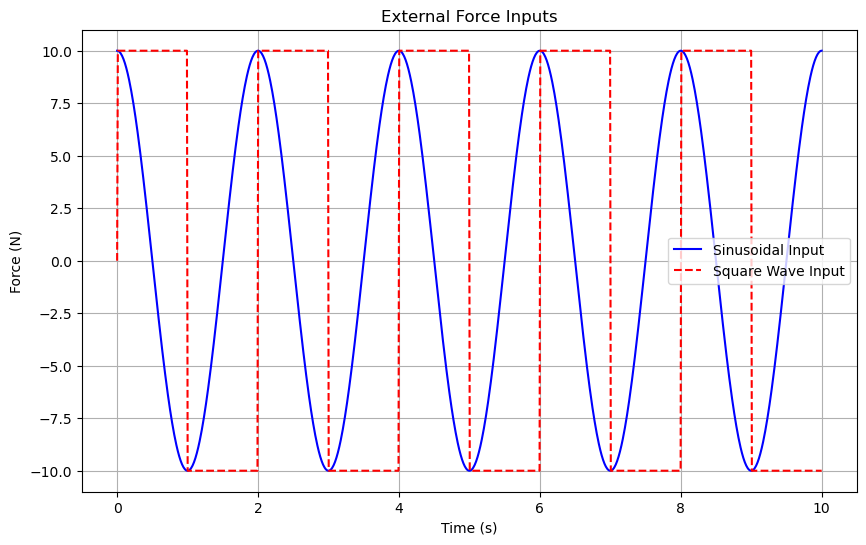
\includegraphics[width=0.8\textwidth]{force_input.png} 
    \caption{External Force Input}
    \label{fig:system}
\end{figure}
{\vspace{10pt}}

The graph shows the external force input to the system, represented as square and sinusodial wave. The square wave alternates between two values, creating a periodic excitation that changes abruptly at specific intervals. This type of excitation can be used to simulate real-world scenarios where the system is subjected to sudden changes in force or pressure. The sinusoidal wave, on the other hand, provides a smooth and continuous excitation that varies sinusoidally over time. This type of excitation is commonly used in vibration analysis to study the system's response to harmonic forces.


{\vspace{10pt}}

\begin{figure}[H]
    \centering
    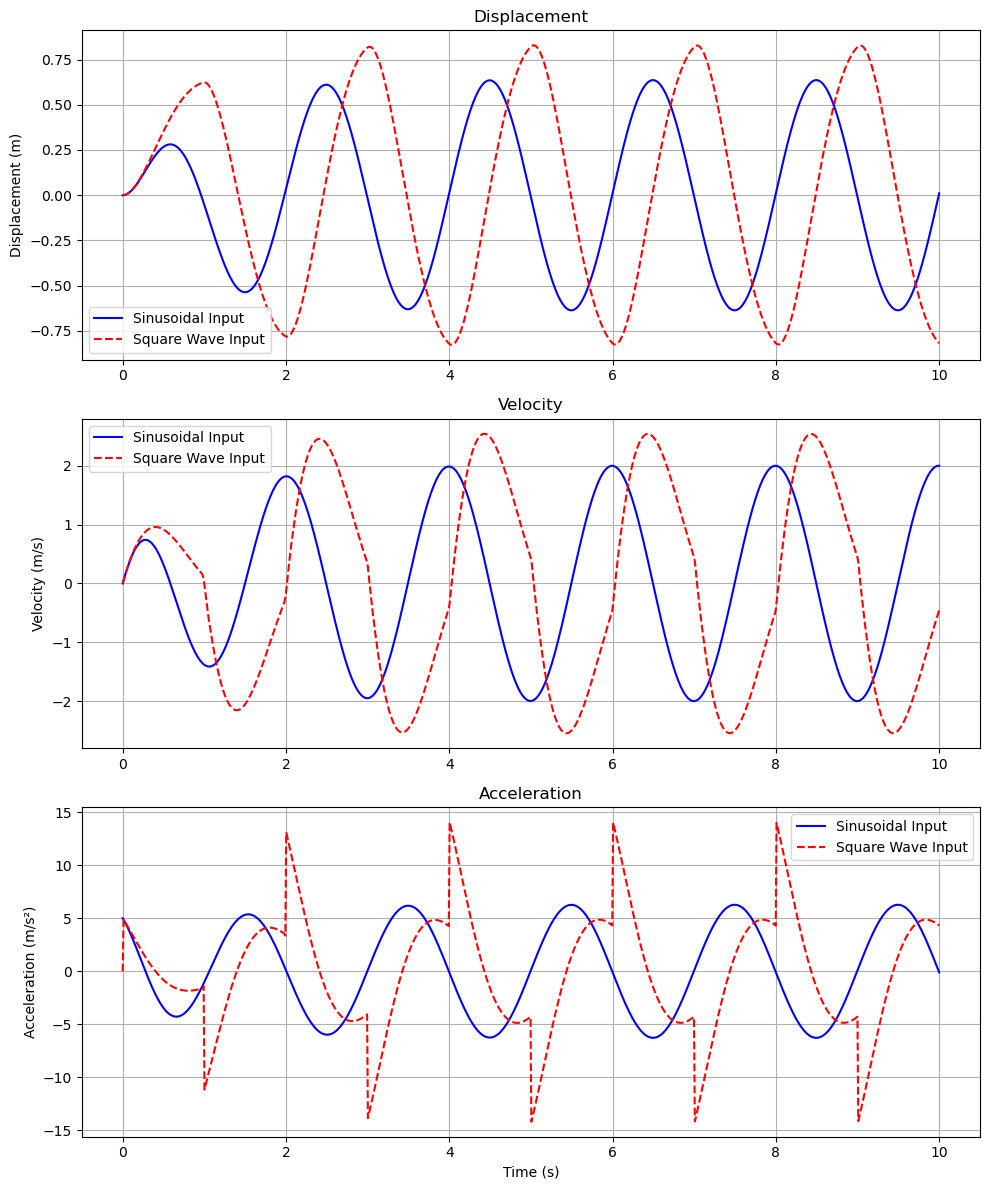
\includegraphics[width=0.8\textwidth]{disp_vel_acc.png  } 
    \caption{Displacement, Velocity and Acceleration }
    \label{fig:system}
\end{figure}
{\vspace{10pt}}

The system’s response to the square wave input exhibits sharp transitions and discontinuities in displacement, velocity, and acceleration, which are characteristic of the abrupt changes in force or pressure applied to the system. The system quickly adjusts to these changes, resulting in oscillations and spikes in the displacement, velocity, and acceleration plots. These behaviors reflect the system's dynamic response to a non-sinusoidal, impulsive force, showing the influence of damping and the system’s natural frequency.
\vspace{5pt}

\noindent\textbf{Displacement Plot }  

When the square wave switches between two values (e.g., 0 and a constant force), the displacement shows sharp transitions. These transitions occur because the system responds immediately to the change in force, causing a quick adjustment in its position. The displacement jumps abruptly at the moments when the force switches. Between these transitions, the displacement remains constant during periods when the force stays constant (either "on" or "off"). This results in plateaus in the displacement plot, where the system holds its position until the force changes again.  
\vspace{5pt}  

\noindent\textbf{Velocity Plot}  

The velocity plot shows sharp peaks when the force switches between its two values, as the velocity is the derivative of displacement. The sudden change in displacement (from one value to another) causes a corresponding spike in velocity. These abrupt velocity changes occur at the moments when the square wave switches. If the displacement changes direction, the velocity will experience a sudden reversal. At the points where the force switches, the system’s direction of motion changes, resulting in a sharp change in the velocity's sign (from positive to negative or vice versa. Like displacement, the velocity also oscillates (but at a higher frequency). The oscillations are more pronounced in velocity because it is the first derivative of displacement. If the system is oscillating under the square wave excitation, the velocity will show higher frequency fluctuations, reflecting the quick changes in speed.
\vspace{5pt}

\noindent\textbf{Acceleration Plot}

The acceleration plot shows the most pronounced discontinuities. Since acceleration is the derivative of velocity, any sharp changes in velocity will create large spikes in the acceleration curve. These spikes are due to the instantaneous changes in velocity caused by the switching force. At the exact moments when the square wave switches, the acceleration will show sharp spikes. These spikes occur because the velocity changes instantaneously, and acceleration is a measure of how quickly the velocity is changing. Acceleration is the second derivative of displacement, which makes it very sensitive to high-frequency changes. Therefore, the acceleration shows higher frequency oscillations than displacement and velocity, reflecting the system's response to the rapid changes in force.
{\vspace{10pt}}

\subsubsection{Frequency Domain Analysis}
\begin{figure}[H]
    \centering
    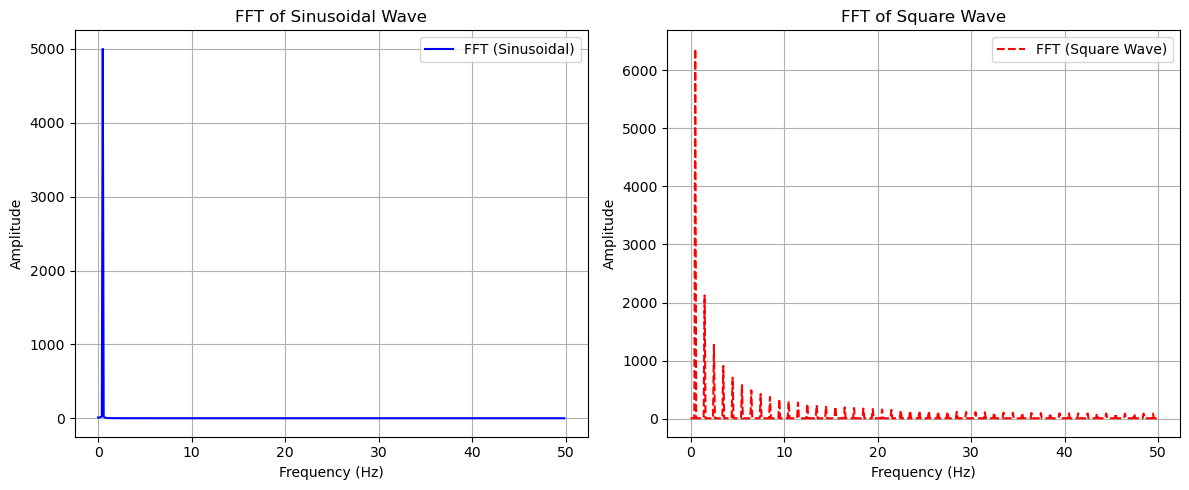
\includegraphics[width=0.8\textwidth]{freq_domain.png} 
    \caption{Frequency Domain Analysis}
    \label{fig:system}
\end{figure}
{\vspace{10pt}}

In the frequency domain, the response of the system under sinusoidal and square wave forcing functions reveals distinct characteristics. For the sinusoidal forcing function, the FFT displays a single dominant peak at the fundamental frequency, corresponding to the oscillatory nature of the input signal. This reflects the fact that a sinusoidal forcing function contains energy concentrated at only one frequency, which simplifies the system's excitation and response.

In contrast, the square wave forcing function produces a more complex frequency spectrum. The FFT of the square wave shows a prominent peak at the fundamental frequency, along with additional peaks at odd harmonics of the fundamental (\( 3f_0, 5f_0, 7f_0, \dots \)). These harmonics arise due to the Fourier series decomposition of the square wave, which contains multiple frequency components.

The square wave forcing distributes energy across a broad range of frequencies, exciting the system not only at the fundamental frequency but also at higher harmonics. This differs significantly from the sinusoidal forcing, which excites the system only at the fundamental frequency. The broader frequency content of the square wave means that the system is subject to a more diverse excitation profile.


{\vspace{10pt}}

\section{Part 2: Base Motion in the Rocket}

\subsection{System Sketch and Representation}
\begin{figure}[H]
    \centering
    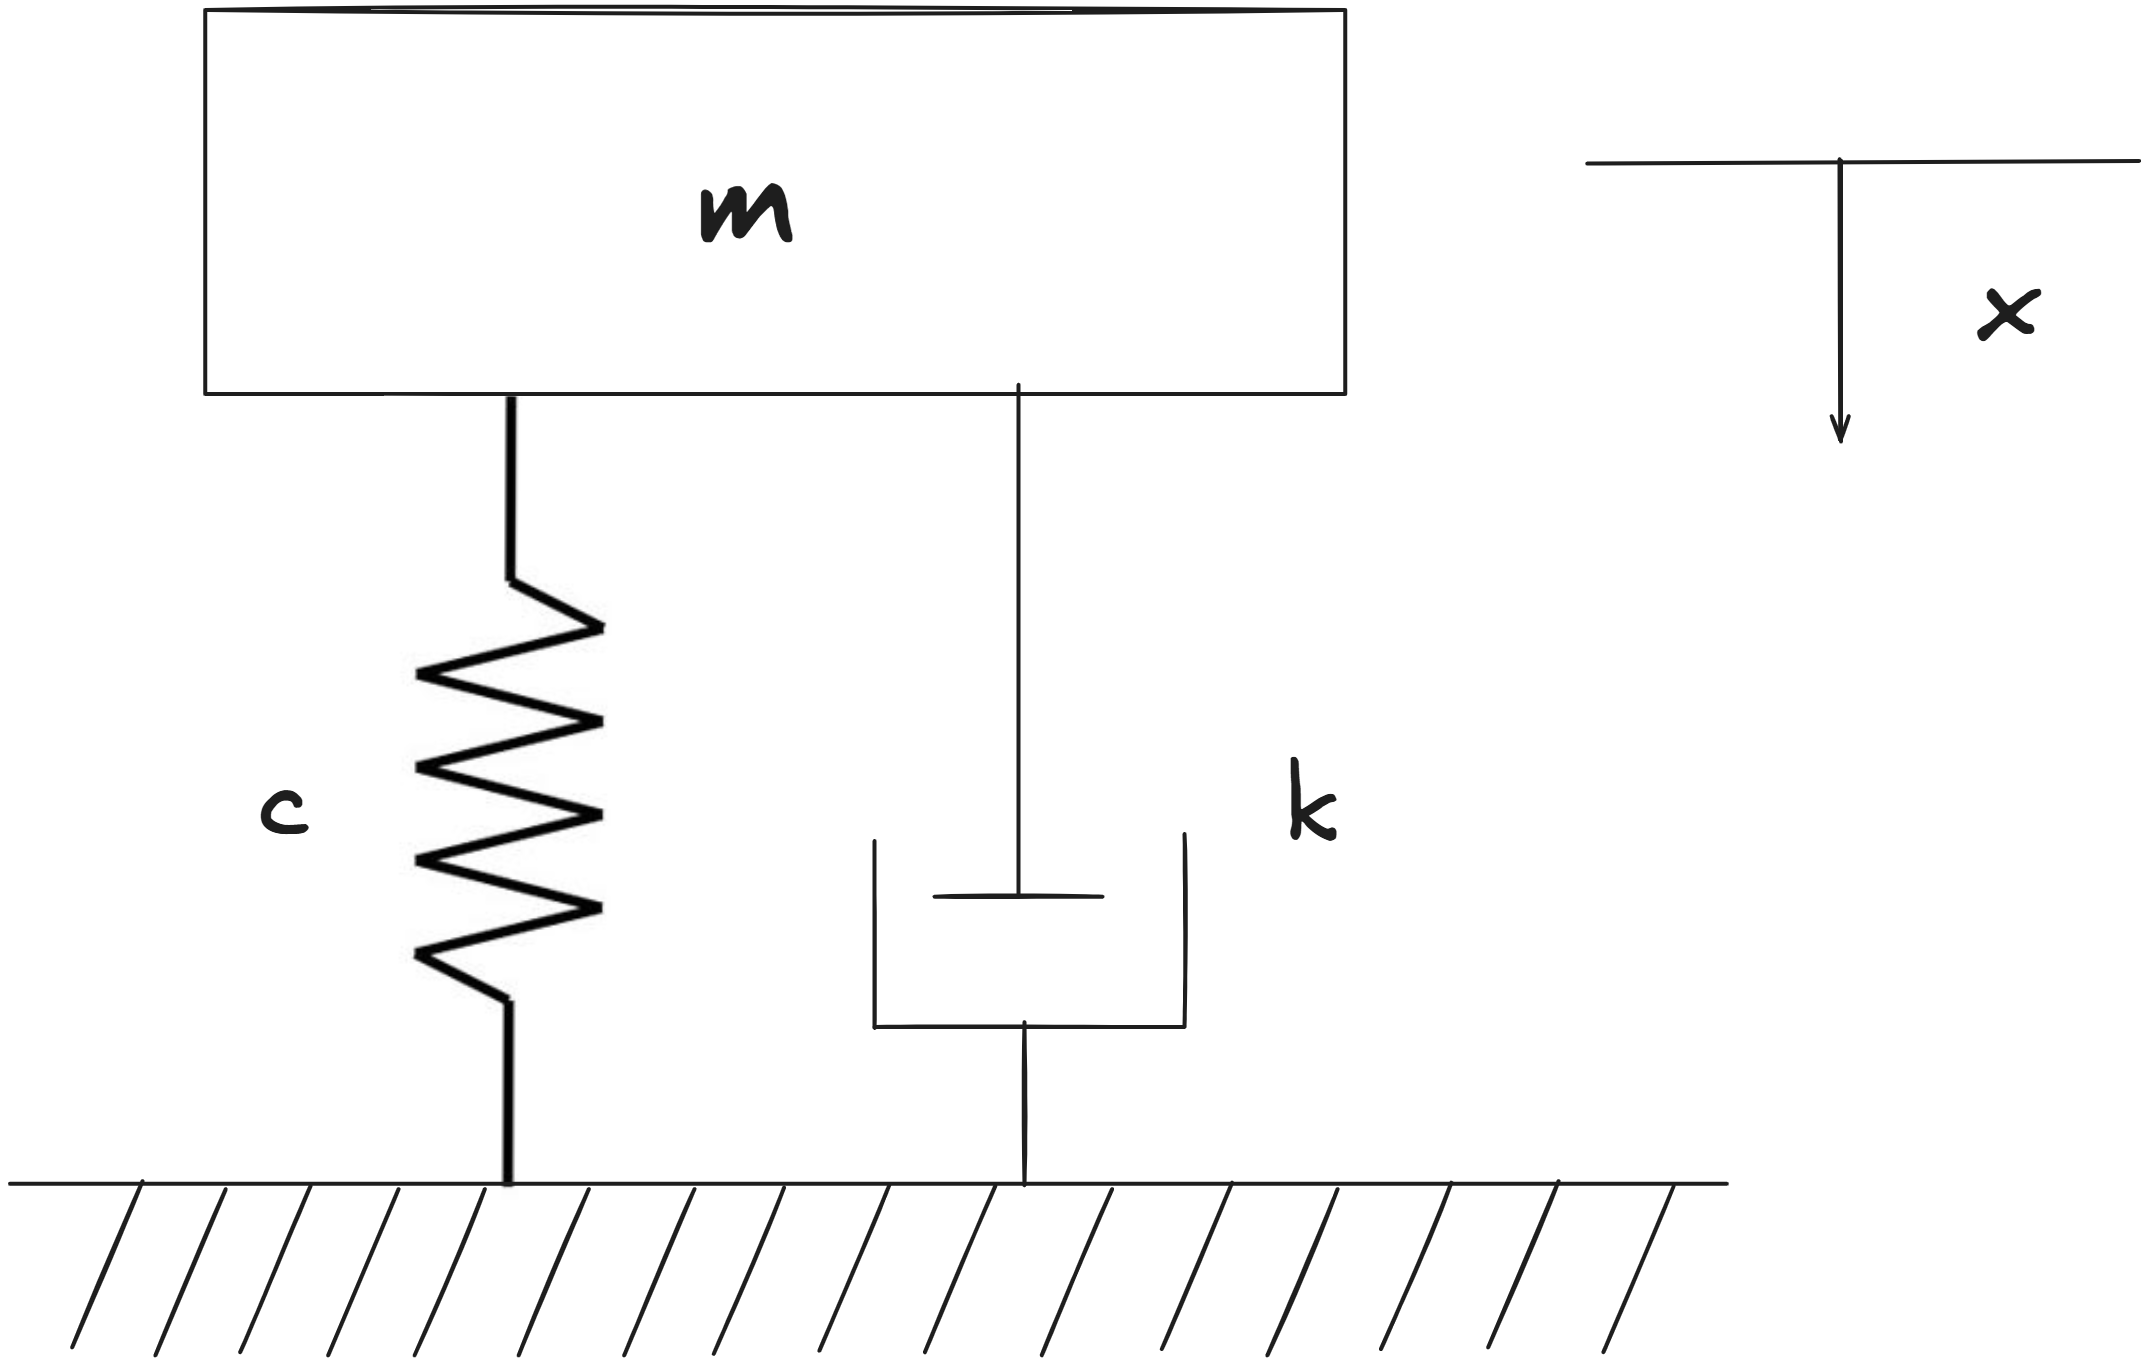
\includegraphics[width=0.8\textwidth]{msd.png} 
    \caption{Mass-Spring-Damper System.}
    \label{fig:system}
\end{figure}
\textbf{Where:}
\begin{itemize}
    \item Spring constant, \(c = 20 \, \text{N/m}\)
    \item Damping constant, \(k = 5 \, \text{Ns/m}\)
    \item Mass, \(m = 5 \, \text{kg}\)
    \item Initial position, \(x = 10 \, \text{m}\)
\end{itemize}

\subsection{Damped and Undamped Responses}
\begin{figure}[H]
    \centering
    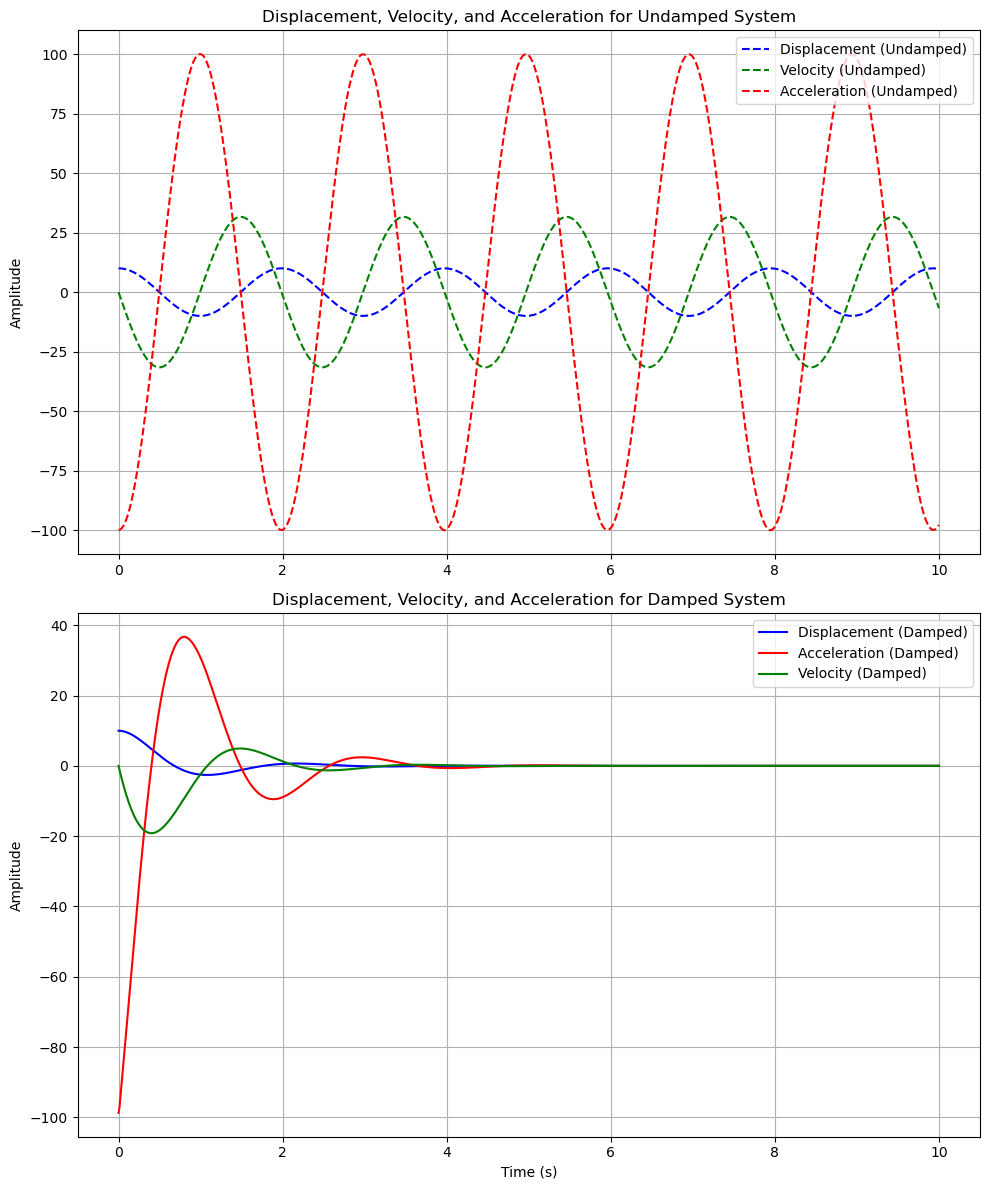
\includegraphics[width=0.8\textwidth]{disp_vel_acc_damp_and_undamp.png} 
    \caption{Displacement, Velocity and acceleration for Damped and Undamped system.}
    \label{fig:system}
\end{figure}
{\vspace{10pt}}
\noindent \textbf{Top Plot: Undamped System}\\
The system is oscillating without any resistance, meaning it continues indefinitely without losing energy. Three different curves are shown:

\begin{itemize}
    \item \textbf{Blue (Displacement)}: This shows how the position of the system changes over time. It oscillates smoothly like a wave, indicating back-and-forth movement.
    \item \textbf{Green (Velocity)}: The velocity (speed and direction) also oscillates, but it's shifted relative to the displacement. It peaks when the displacement crosses zero, as the system is moving the fastest.
    \item \textbf{Red (Acceleration)}: The acceleration, representing the change in velocity, also oscillates but with a larger amplitude than the others. It peaks at the extremes of displacement, where the system has the maximum force applied to it.
\end{itemize}

\noindent The undamped system oscillates with the same amplitude continuously because there's no friction or damping to reduce the motion.

{\vspace{10pt}}
\noindent \textbf{Bottom Plot: Damped System}\\
This shows a system where damping is present, meaning there's resistance that reduces the oscillation over time.

\begin{itemize}
    \item The curves for displacement (\textbf{blue}), velocity (\textbf{green}), and acceleration (\textbf{red}) are initially similar to the undamped system but start to decrease in amplitude as time goes on.
    \item The system eventually settles down to a stable point where there is no motion (equilibrium). This happens because the damping absorbs the energy from the system, causing the oscillations to die out over time.
\end{itemize}

{\vspace{10pt}}

\subsection{Mass Spring Damper with moving Base}
\begin{figure}[H]
    \centering
    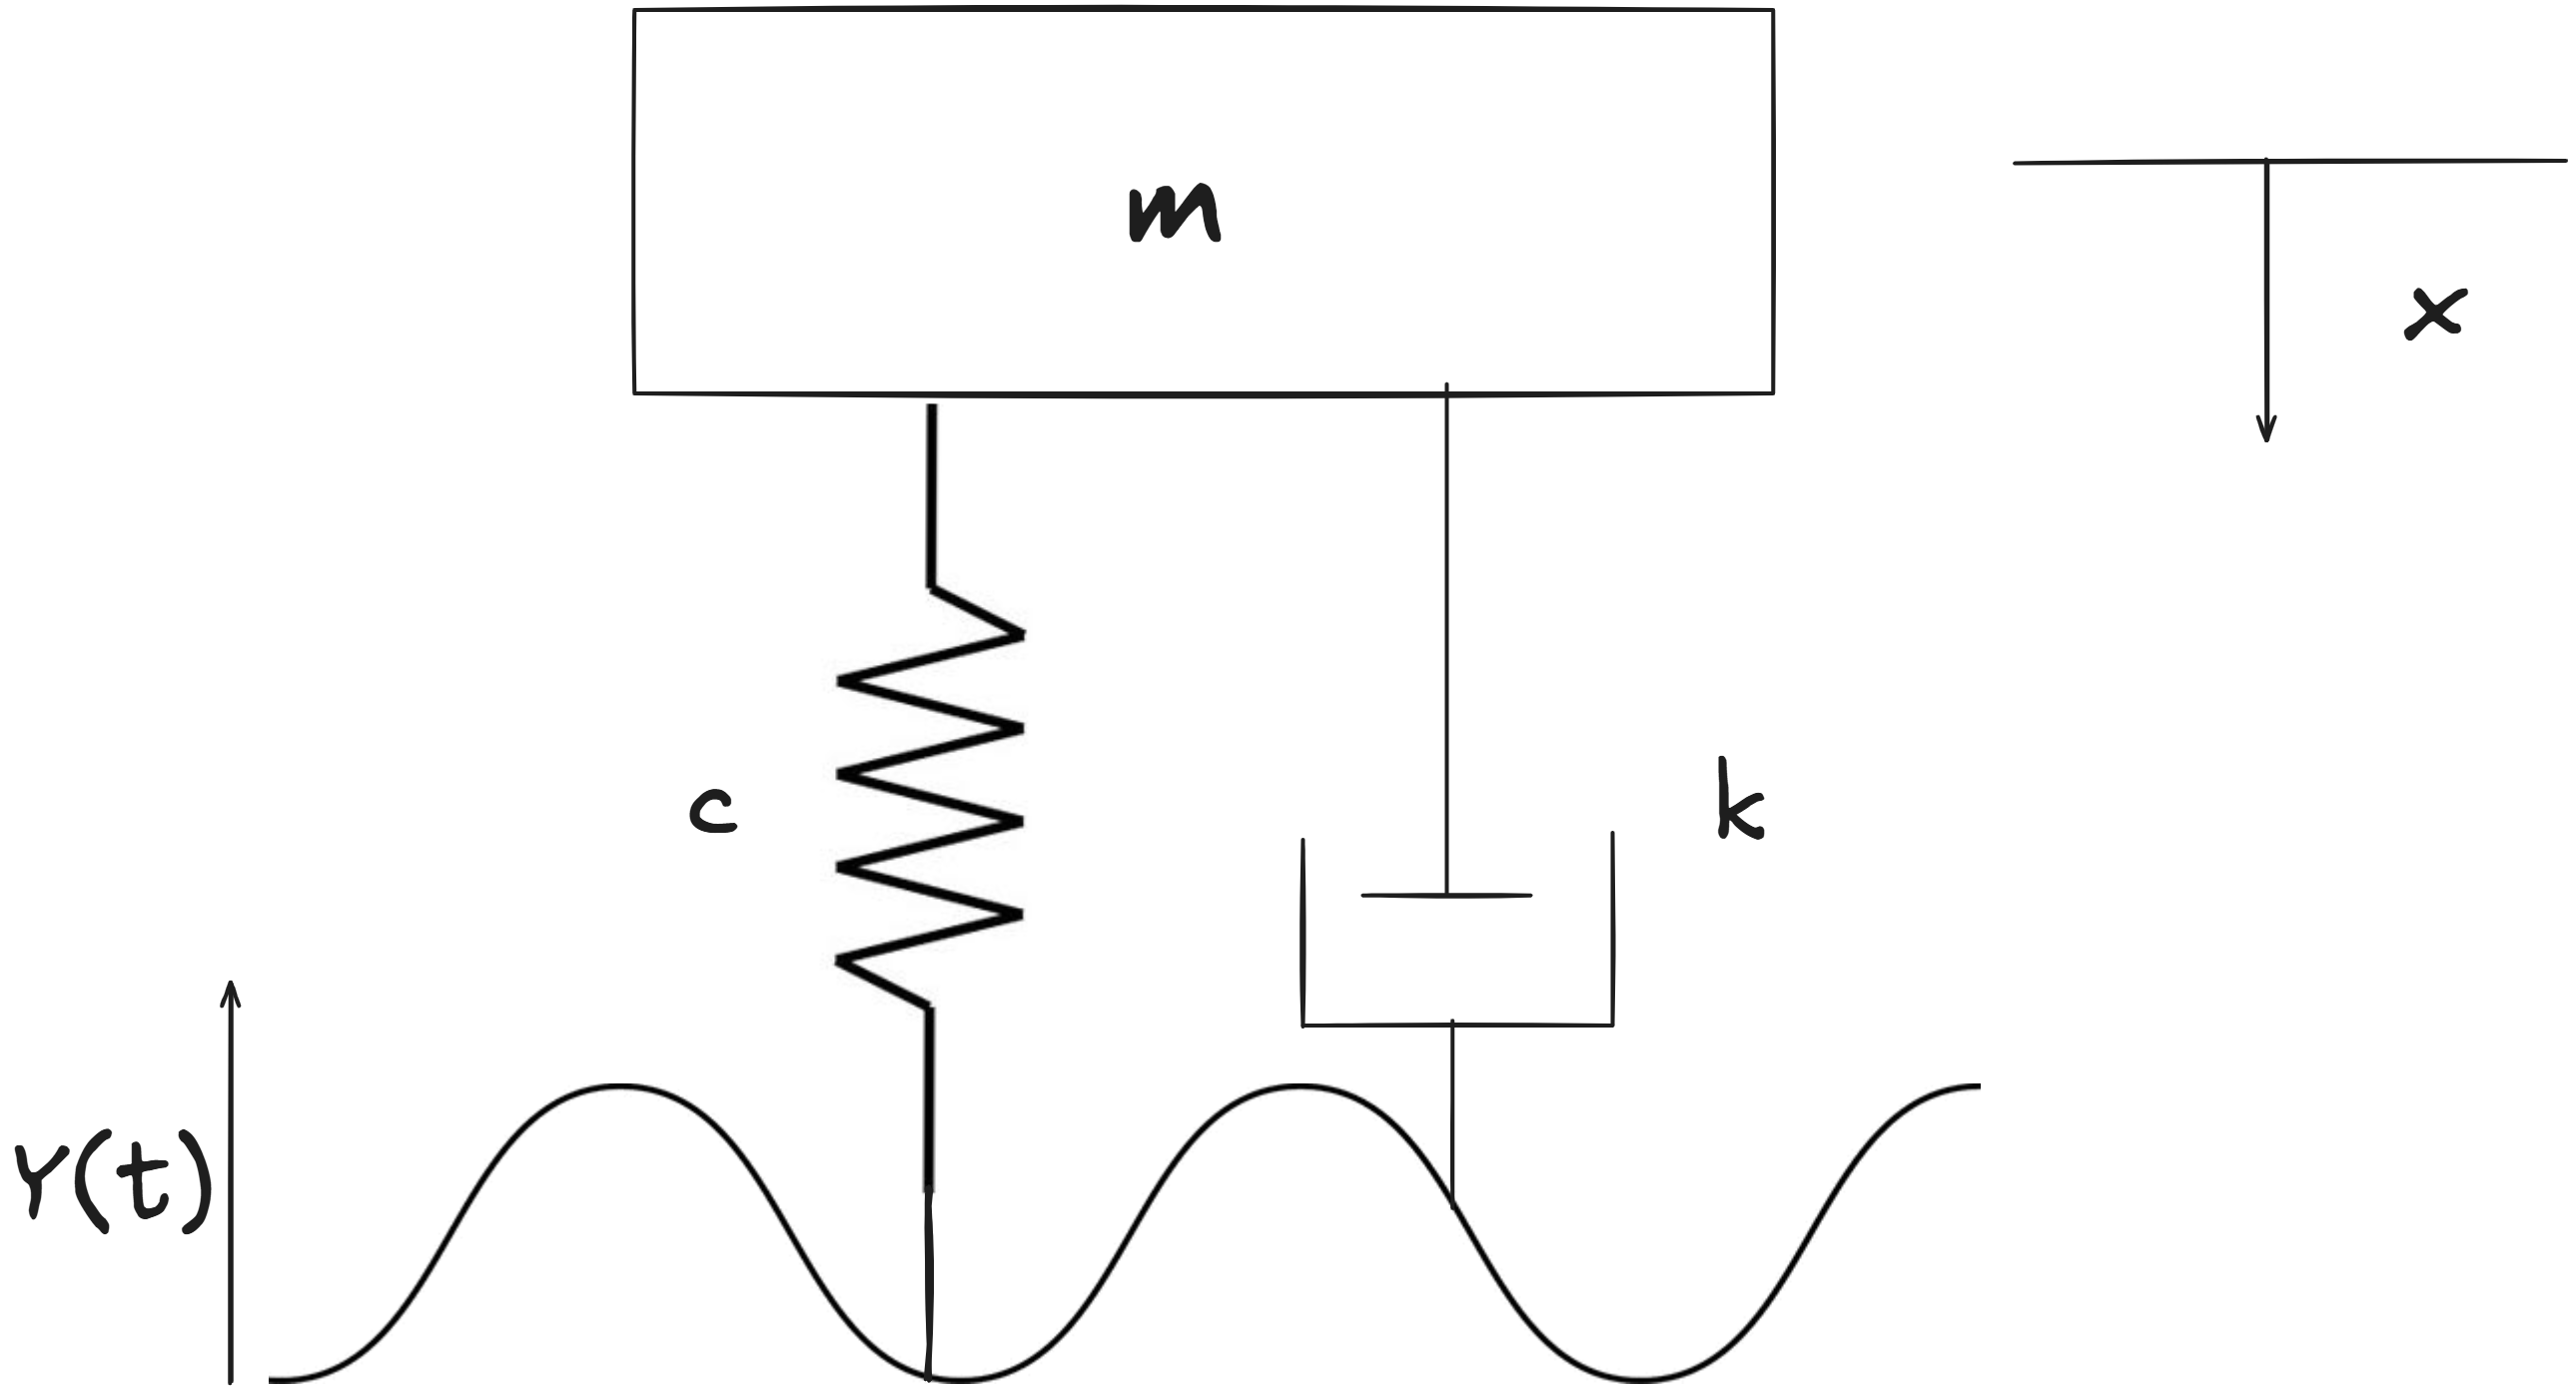
\includegraphics[width=0.8\textwidth]{msd_base.png} 
    \caption{Mass-Spring-Damper system with moving base.}
    \label{fig:system}
\end{figure}
\textbf{Where:}
\begin{itemize}
    \item Mass, \(m = 5 \, \text{kg}\)
    \item Spring constant, \(c = 20 \, \text{N/m}\)
    \item Damping constant, \(k = 5 \, \text{Ns/m}\)
    \item Initial position, \(x = 10 \, \text{m}\)
    \item Base Force, \(Y(t) = Y_0 \cos(\omega t)\)    
\end{itemize}
{\vspace{5pt}}
The system above represents a \textbf{mass-spring-damper} system with a moving base. The base force \(Y(t)\) is a harmonic function with amplitude \(Y_0\) and angular frequency \(\omega\). The system's response is influenced by the base motion, which can lead to interesting behaviors such as resonance, phase shifts, and amplitude changes.

{\vspace{5pt}}

\subsection{Amplitude and Phase Angle}

Calculating Amplitude and Phase Angle:  

{\vspace{5pt}}

\textbf{Given:}

- Base Excitation Force: 
\[
Y(t) = Y_0 \cos(\omega t)
\]
\[
\dot{Y}(t) = -\omega Y_0 \sin(\omega t)
\]

- Angular Frequency: 
\[
\omega = \frac{2 \pi}{l}
\]

\textbf{Given:}
\begin{itemize}
    \item \( V = 2000 \, \text{m/s} \)
    \item \( l = 1000 \, \text{m} \)
\end{itemize}

\[
\omega = 12.566 \, \text{rad/s}
\]

The system model is given by:

\[
m \ddot{x}  + k \dot{x} + c x = y(t)
\]

where:
\begin{itemize}
    \item \( m = \text{Mass} \)
    \item \( k = \text{Damping Constant} \)
    \item \( c = \text{Spring Constant} \)
    \item \( x = \text{Displacement} \)
    \item \( \dot{x} = \text{Velocity} \)
    \item \( \ddot{x} = \text{Acceleration} \)
    \item \( Y(t) = Y \cos(\omega t) \)
\end{itemize}

{\vspace{5pt}}

From Newton's Second Law, \( \sum F = ma \), we have:

\[
m \ddot{x} + k (\dot{x} - \dot{Y}) + c(x - Y) = 0
\]
\[
m \ddot{x} + k \dot{x} - k \dot{Y} + c x - cY = 0
\]
\[
m \ddot{x} + k \dot{x} + c x = c Y + k \dot{Y}
\]

{\vspace{5pt}}

Substituting for \( y \) and \( \dot{y} \), we have:

\[
m \ddot{x} + k \dot{x} + c x = c Y \cos(\omega t) - k \omega Y \sin(\omega t)
\]

{\vspace{5pt}}

We know that:

\[
x = X_0 \cos(\omega t - \phi) \quad \text{(eq. 1)}
\]
\[
\dot{x} = -\omega X_0 \sin(\omega t - \phi) \quad \text{(eq. 2)}
\]
\[
\ddot{x} = -\omega^2 X_0 \cos(\omega t - \phi) \quad \text{(eq. 3)}
\]

{\vspace{5pt}}

Substituting eq. (1), eq. (2), and eq. (3) into the system model, we have:

\[
m (-\omega^2 X_0 \cos(\omega t - \phi)) + k (-\omega X_0 \sin(\omega t - \phi)) + c (X_0 \cos(\omega t - \phi)) = c Y \cos(\omega t) - k \omega Y \sin(\omega t)
\]

{\vspace{5pt}}

After Phasor representation, we have:

\[
F_{\text{res1}}^2 = c Y^2 + k Y \omega^2
\]
\[
= Y^2 (c^2 + k^2 \omega^2)
\]

\[
F_{\text{res2}}^2 = (k X_0 \omega)^2 + (c X_0 - m X_0 \omega)^2
\]
\[
= X_0^2 \left[ (k \omega)^2 + (c - m \omega^2)^2 \right]
\]

{\vspace{5pt}}

Equating \( F_{\text{res1}}^2 \) and \( F_{\text{res2}}^2 \), we have:

\[
Y^2 (c^2 + k^2 \omega^2) = X_0^2 \left[ (k \omega)^2 + (c - m \omega^2)^2 \right]
\]

{\vspace{5pt}}

Equations for \( X_0 \) and \( \phi \), we have:

\[
X_0 = Y_0 \sqrt{ \frac{c^2 + (k \omega)^2}{(k \omega)^2 + (c - m \omega^2)^2} }
\]

\[
\phi = \tan^{-1}\left( \frac{m \omega^3 k}{c^2 - m \omega^2 c + k^2 \omega^2} \right)
\]

{\vspace{5pt}}

Solving for \( X_0 \) and \( \phi \):

Given:
\begin{itemize}
    \item \( m = 2 \, \text{kg} \)
    \item \( k = 5 \, \text{N/m} \)
    \item \( c = 20 \, \text{Ns/m} \)
    \item \( Y_0 = 150 \, \text{m} \)
    \item \( \omega = 12.566 \, \text{rad/s} \)
\end{itemize}

{\vspace{5pt}}

We have:

\[
X_0 = 151 \sqrt{ \frac{20^2 + (5 \times 12.566)^2}{(5 \times 12.566)^2 + (20 - 2 \times (12.566)^2)^2} }
\]

\[
\phi = \tan^{-1}\left( \frac{2 \times (12.566)^3 \times 5}{20^2 - 2 \times (12.566)^2 \times 20 + 5^2 \times (12.566)^2} \right)
\]

{\vspace{5pt}}

Thus:

\[
X_0 = 32.92 \, \text{m}
\]
\[
\phi = -84.334 \, \text{rad/s} \quad (95.67^\circ)
\]

{\vspace{5pt}}

\subsection{State Space Representation}
The general State-Space Representation of a second order system is:
\[
\dot{X} = \underset{\rightarrow}{A}\vec{x} + \underset{\rightarrow}{B}\vec{u}
\]

Introduce the state variables:
\[
x_1 = x, \quad x_2 = \dot{x}
\]

This gives:
\[
\dot{x}_1 = x_2, \quad \dot{x}_2 = \ddot{x}
\]

From the differential equation:
\[
m\ddot{x} = -k\dot{x} - cx + k\dot{Y} + cY
\]

Re-arranging for \( \ddot{x} \):
\[
\dot{x}_2 = -\frac{c}{m}x_1 - \frac{k}{m}x_2 + \frac{k}{m}\dot{Y} + \frac{c}{m}Y
\]

Now, the state-space form becomes:
\[
\begin{bmatrix}
\dot{x}_1 \\
\dot{x}_2
\end{bmatrix}
=
\underbrace{
\begin{bmatrix}
0 & 1 \\
-\frac{c}{m} & -\frac{k}{m}
\end{bmatrix}}_{A}
\begin{bmatrix}
x_1 \\
x_2
\end{bmatrix}
+
\underbrace{
\begin{bmatrix}
0 & 0 \\
\frac{c}{m} & \frac{k}{m}
\end{bmatrix}}_{B}
\begin{bmatrix}
Y \\
\dot{Y}
\end{bmatrix}
\]

Here:
\begin{itemize}
    \item \( A \) is the system matrix.
    \item \( B \) accounts for the influence of \( Y(t) \) and \( \dot{Y}(t) \), the base motion and its velocity.
\end{itemize}

Substituting the values:
\[
\begin{bmatrix}
\dot{x}_1 \\
\dot{x}_2
\end{bmatrix}
=
\begin{bmatrix}
0 & 1 \\
-10 & -2.5
\end{bmatrix}
\begin{bmatrix}
x_1 \\
x_2
\end{bmatrix}
+
\begin{bmatrix}
0 & 0 \\
10 & 2.5
\end{bmatrix}
\begin{bmatrix}
Y \\
\dot{Y}
\end{bmatrix}
\]

\vspace{5pt}

Base excitation only influences the second state equation because it directly affects the system's forces, which in turn affects the acceleration. The first state equation describing the relationship between Displacement and velocity is not influenced by external input.

The systems dynamics are influenced by the relative motion between the mass and the base. This is becasue the base excitation directly acts as an external force or input that impacts the systems dynamics through its velocity with the mass and spring. 



\subsection{Impact of Base Excitation Amplitude}
\begin{figure}[H]
    \centering
    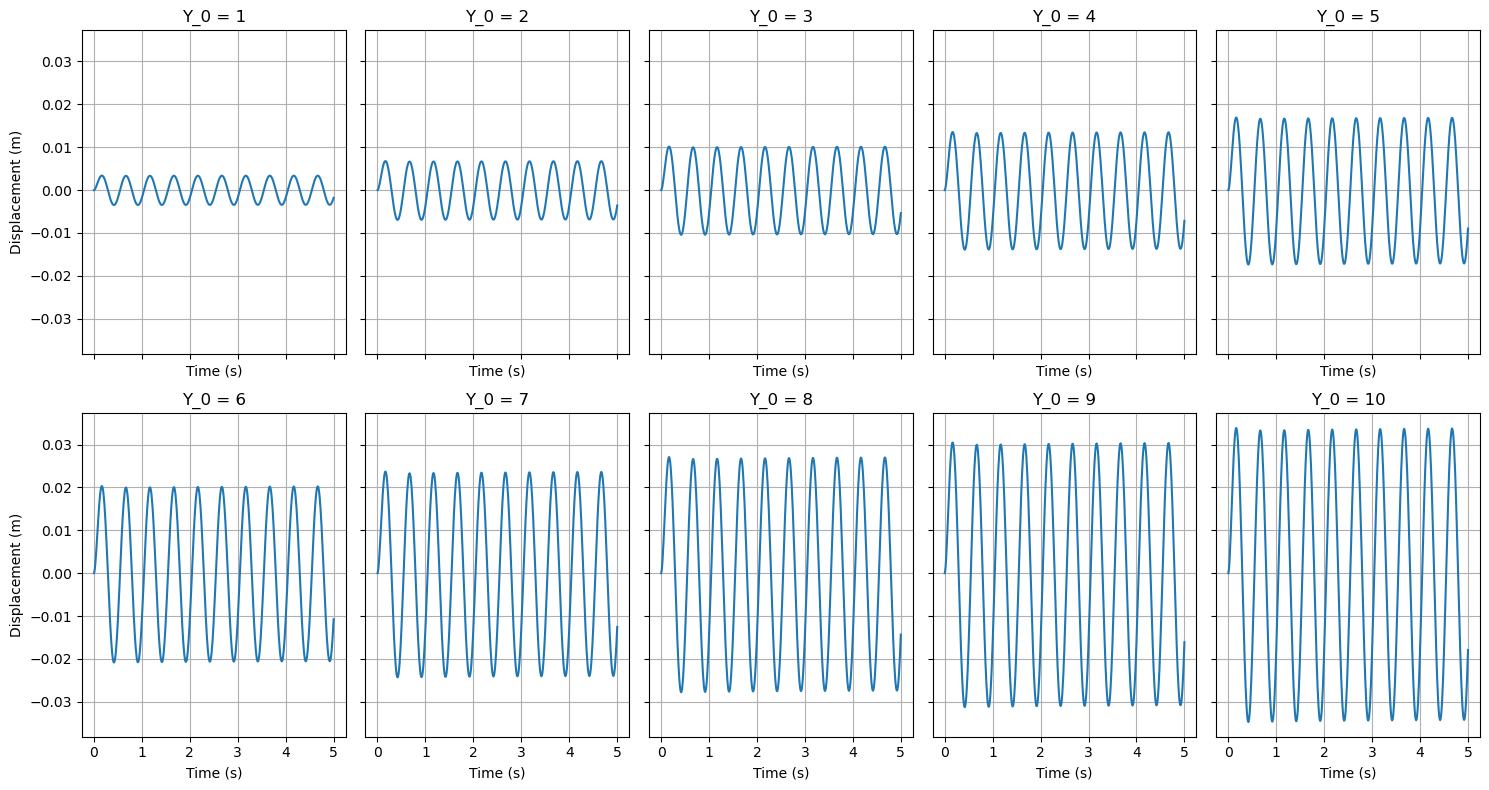
\includegraphics[width=0.8\textwidth]{disp_response.png} 
    \caption{Displacement Response for different Y0 values}
    \label{fig:system}
\end{figure}
{\vspace{10pt}}


The graph shows how the system's displacement response changes over time for various base excitation amplitudes (\(Y_0\)). As \(Y_0\) increases, the amplitude of the displacement response also increases proportionally. This is expected because the system's displacement is directly influenced by the amplitude of the base excitation. The periodic nature of the displacement response indicates that the system follows the excitation frequency (\(\omega\)), maintaining a consistent oscillatory behavior.

When a vehicle drives over uneven roads, such as potholes or speed bumps, the suspension system is designed to absorb these irregularities. If the displacement response of the suspension system is too large, passengers will experience uncomfortable vibrations and jolts.

By analyzing how the suspension responds to different road conditions (which can be modeled as base excitations like \(Y_0\)), engineers can fine-tune the suspension to ensure that the vehicle's body does not excessively move, keeping the ride smooth and stable.




{\vspace{10pt}}

\begin{figure}[H]
    \centering
    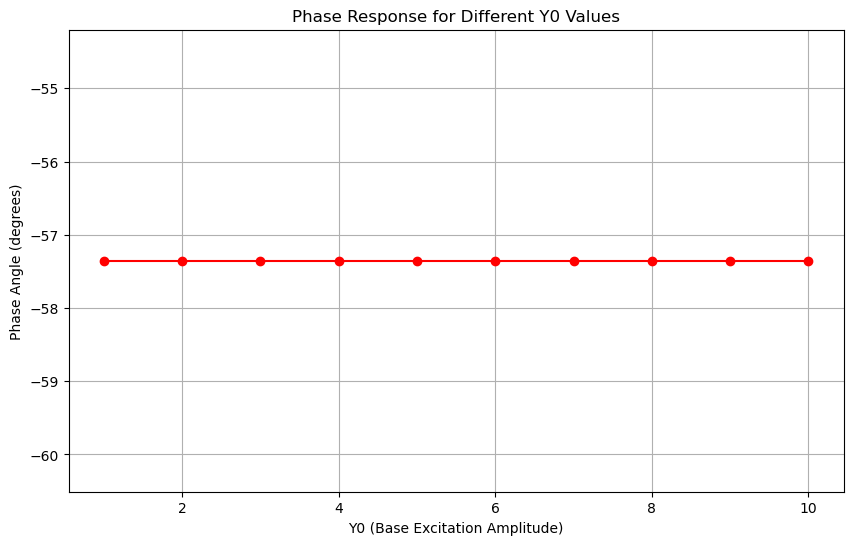
\includegraphics[width=0.8\textwidth]{phase_resp.png} 
    \caption{Phase Response for different Y0 values}
    \label{fig:system}
\end{figure}
{\vspace{10pt}}
The phase angle remains nearly constant across all \(Y_0\) values. This shows that the system's phase relationship with the excitation does not depend on the amplitude of the base excitation. The phase response is a function of the system's natural frequency, damping ratio, and excitation frequency. Since these parameters remain unchanged, the phase angle does not vary with \(Y_0\).

The phase response is related to the timing of a vehicle's body movement in relation to the road disturbances. If the suspension system has a poor phase response, it may lag too much or move out of sync with the road, causing instability or resonance.

For example, during high-speed travel, if the suspension's phase angle is not properly tuned, it could amplify vibrations rather than dampen them, making the vehicle harder to control and less safe.

{\vspace{10pt}}

{\vspace{5pt}}
The displacement response scales with the excitation amplitude, but the phase response is independent of \(Y_0\).
This behavior is typical for linear systems, where the system's response to an input is directly proportional to the input amplitude, and the phase depends only on the system dynamics and excitation frequency.

By analyzing and optimizing both the displacement and phase responses, engineers can design vehicles that minimize vibrations and jolts for a comfortable ride and ensure the vehicle remains stable and controllable under dynamic conditions like sudden turns, braking, or uneven terrain.
{\vspace{5pt}}

    
\end{document}
